%
% Kurvenintegral einer 1-Form
%
\section{Kurvenintegral einer 1-Form
\label{buch:kurvenintegral:section:1form}}
\kopfrechts{Kurvenintegral einer 1-Form}%
Eine Kurve ist eine eindimensionale Untermannigfaltigkeit in
einer $n$-dimensionalen Mannigfaltigkeit $M$.
Eine $1$-Form auf der Mannigfaltigkeit $M$ führt zu einer 
$1$-Form auf der Kurve und damit wird es möglich, das Integral
dieser 1-Form auf der Kurve zu berechnen.
Dies soll in diesem Abschnitt schrittweise durchgeführt werden.

%
% 1-Form auf einer Mannigfaltigkeit
%
\subsection{$1$-Form auf einer Mannigfaltigkeit}
Eine $1$-Form auf einer $n$-dimensionalen Mannigfaltigkeit ist eine
Linearform, die auf einen Tangentialvektor angewendet werden kann
und einen Zahlenwert ergibt.
In einem Koordinatensystem mit den Koordinaten $x^1,\dots,x^n$ bilden
die Tangentialvektoren an die Koordinatenlinien eine Basis des
Tangentialraumes.
Die einzelnen Basisvektoren sind früher schon mit den
Ableitungsoperatoren $\partial/\partial x^i$ identifiziert worden.
Die Koordinaten-1-Formen $dx^1,\dots,dx^n$ ermitteln, wie schnell sich
die entsprechende Koordinate entlang eines Tangentialvektors ändert.
Da sich entlang einer Koordinatenlinie immer nur eine einzige
Koordinate ändert, gilt
\[
\biggl\langle dx^i,\frac{\partial}{\partial x^k}\biggr\rangle
=
\delta_{ik}
=
\begin{cases}
1&\qquad \text{falls $i=k$}\\
0&\qquad \text{sonst}.
\end{cases}
\]
\index{<,>@$\langle\;\,,\;\rangle$}%
Man nennt diese Basis der Linearformen auch die zur Basis der
Ableitungsoperatoren \emph{duale Basis}.

Eine $1$-Form auf der Mannigfaltigkeit hat daher im Koordinatensystem
mit den Koordinaten $x^i$ die Form
\[
\alpha
=
\alpha_i(x)\, dx^i,
\]
wobei wieder die Summationskonvention gilt.

\begin{beispiel}
Die $1$-Form
\[
\beta
=
-
\sum_{i=1}^n
\frac{GMx^i}{r^3}
dx^i
\]
soll auf dem Impulsvektor eines Teilchens berechnet werden.
Die Summationskonvention ist hier nicht anwendbar, da der Index $i$ zweimal
als oberer Index auftritt.
\index{Impuls}%
Wird die Bahnkurve mit der Zeit parametrisiert, hat der Geschwindigkeitsvektor
die Komponenten $\dot{x}^i$.
Der Impuls $p$ des Teilchens ist der Vektor mit den Komponenten
$p^i=m\dot{x}^i$.
Wendet man die Linearform $\beta$ darauf an, ergibt sich
\begin{align}
\langle \alpha, p\rangle
&=
-
\frac{GMm}{r^3}
\biggl\langle \sum_i x^i\,dx^i, \sum_k\dot{x}^k\frac{\partial}{\partial x_k}\biggr\rangle
=
-
\frac{GMm}{r^3}
\sum_{i,k} x^i \biggl\langle dx^i,\dot{x}^k\frac{\partial}{\partial x_k}\biggr\rangle
\notag
\\
&=
-
\frac{GMm}{r^3}
\sum_{i,k}
x^i \delta_{ik} \dot{x}^k
=
-\frac{GMm}{r^3}
\sum_i x^i\dot{x}^i
\label{buch:kurvenintegral:kurvenintegral:eqn:gravimpuls}
\end{align}
Dies ist die Leistung, die das Teilchen gegen das Gravitationsfeld 
arbeitet.
Eine $1$-Form ist also dazu geeignet, ein wichtiges physikalisches Konzept
des Gravitationsfeldes auszudrücken.
\end{beispiel}

Die Form
\eqref{buch:kurvenintegral:kurvenintegral:eqn:gravimpuls}
ist allerdings noch nicht wirklich geeignet.
In der Formel wurden kontravariante Komponenten miteinander multipliziert
und summiert, dies führt nicht auf eine koordinatensystemunabhängige
Grösse.
Dazu müssten aus einem oberen Index in unterer gemacht werden können
oder umgekehrt.
Mit einer Metrik ist dies möglich, wie die musikalischen Operationen
gemäss
Definition~\ref{buch:kurvenintegral:differential:def:musikalisch}
zeigen.

%
% Abbildung auf einer $1$-Form
%
\subsection{Abbildung einer $1$-Form}
Sei wieder eine $1$-Form $\alpha$ auf einer $n$-dimensionalen Mannigfaltigkeit
durch die Koeffizienten $\alpha_i(x)$ gegeben.
Sei ausserdem $f\colon N\to M$ eine differenzierbare Abbildung einer
$m$-dimensionalen Mannigfaltigkeit $N$ in die Mannigfaltigkeit $M$.
Ein Tangentialvektor von $N$ im Punkt $p$ wird dargestellt durch eine
Kurve durch den Punkt $p$ in $N$.
Durch die Abbildung $f$ wird die Kurve auf eine Kurve durch den Bildpunkt
$q=f(p)$ abgebildet.
Da die Abbildung $f$ differenzierbar ist, entspricht der Bildkurve 
ein Tangentialvektor im Punkt $f(p)$.
Dies ist die Tangentialabbildung $Tf\colon TN\to TM$, die Tangentialvektoren
von $N$ auf Tangentialvektoren von $M$ abbildet.

Eine $1$-Form berechnet aus einem Tangentialvektor einen Zahlenwert.
Die $1$-Form $\alpha$ auf $M$ tut dies für Tangentialvektoren $X$ von
$M$, nicht aber für Tangentialvektoren von $N$.
Dazu muss erst die Abbildung $Tf$ angewendet werden, die aus dem
Tangentialvektor $Y\in T_pN$ einen Tangentialvektor $T_pf(Y)=X\in T_qM$
macht.
Die Abbildung
\[
Y\mapsto \langle \alpha, T_pf(Y)\rangle \in \mathbb{R}
\]
ist eine lineare Abbildung, denn die Abbildung $T_pf$ ist linear und
Auswertung $X\mapsto \langle\alpha,X\rangle$ ist ebenfalls linear.
Die $1$-Form $\alpha$ auf $M$ definiert damit auch eine $1$-Form auf
$N$, die wir mit $T_pf^*\alpha$ bezeichnen.

\begin{beispiel}
\label{buch:kurvenintegral:kurvenintegral:beispiel:loxodrome}
%
% fig-loxodrome.tex
%
% (c) 2025 Prof Dr Andreas Müller
%
\begin{figure}
\centering
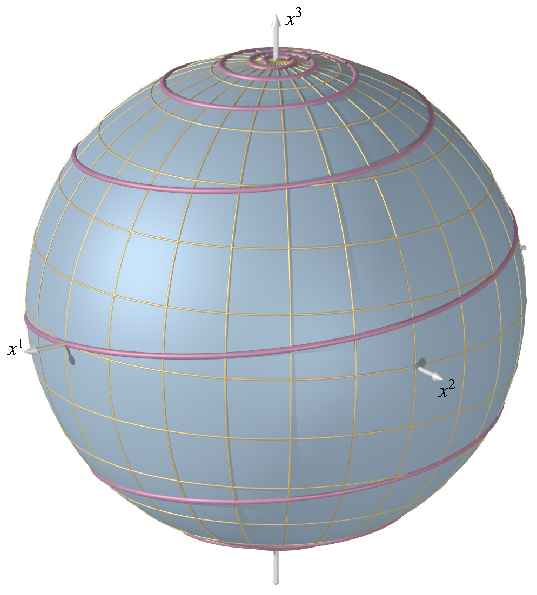
\includegraphics{chapters/030-kurvenintegral/images/loxodrome.pdf}
\caption{Die Loxodrome auf einer Kugeloberfläche schneidet die Längen- und
Breitenkreise unter konstantem Winkel.
Als Abbildung $\mathbb{R}\to S^2$ transportiert die Loxodrome die
$1$-Form $\sin^2\vartheta\,d\varphi$ auf der Kugeloberfläche auf die
reelle Achse und macht daraus die $1$-Form $(1-\tanh^2 kt)\,dt$.
\label{buch:kurvenintegral:fig:loxodrome}}
\end{figure}
%
Sei $N=\mathbb{R}$ eindimensional und $M=S^2$ eine Kugel.
Die Abbildung 
\begin{equation}
f
\colon
\mathbb{R}\to S^2
:
t
\mapsto 
\frac{1}{\cosh kt}
\begin{pmatrix}
\cos t\\
\sin t\\
\sinh kt
\end{pmatrix}
\label{buch:kurvenintegral:kurvenintegral:eqn:kugel}
\end{equation}
beschreibt eine Kurve auf der Kugeloberfläche, die als die
\emph{Loxodrome} bekannt ist.
\index{Loxodrome}%
Sie schneidet die Längenkreise unter konstantem Winkel $\arctan k$
(Abbildung~\ref{buch:kurvenintegral:fig:loxodrome}).
Wir betrachten die $1$-Form $\sin^2\vartheta\cdot d\varphi$, wobei
$(\varphi,\vartheta)$ die Längen- und Breitenkoordinaten auf der
Kugeloberfläche sind.

Um den Tangentialvektor in den $(\varphi,\vartheta)$-Koordinaten zu
bestimmen, muss als erstes der Bildpunkt der Abbildung $f$ in Länge
und Breite umgerechnet werden.
Zunächst kann man aus der Darstellung
\eqref{buch:kurvenintegral:kurvenintegral:eqn:kugel}
sofort ablesen, dass $t=\varphi$ die geographische Länge ist,
es bleibt also nur noch die geographische Breite zu bestimmen.
Diese lässt sich aber sofort aus der $z$-Komponente ablesen:
\[
\cos\vartheta
=
z
=
\frac{\sinh kt}{\cosh kt}
=
\tanh kt
\qquad\Rightarrow\qquad
\vartheta = \arccos\tanh kt.
\]
Damit kann jetzt der Tangentialvektor berechnet werden, werden:
\begin{align*}
\frac{d}{dt} \bigl(\varphi(t),\vartheta(t)\bigr)
&=
\biggl(
\frac{d\varphi(t)}{dt},
\frac{d\vartheta(t)}{dt}
\biggr)
\\
&=
\biggl(1,
-\frac{k\operatorname{sech}^2(kt)}{\sqrt{1-\tanh^2(kt)}}
\biggr)
\\
&=
\frac{\partial}{\partial \varphi}
-
\frac{k\operatorname{sech}^2(kt)}{\sqrt{1-\tanh^2(kt)}}
\frac{\partial}{\partial\vartheta}
.
\end{align*}
Damit sind die Komponenten des Tangentialvektors in
$(\varphi,\vartheta)$-Koordinaten gefunden.

Wir wenden jetzt die $1$-Form $\sin^2\vartheta\, d\varphi$ darauf
an und erhalten:
\begin{align*}
\biggl\langle
\sin^2\vartheta\,d\varphi
,
\frac{\partial}{\partial \varphi}
-
\frac{k\operatorname{sech}^2(kt)}{\sqrt{1-\tanh^2(kt)}}
\frac{\partial}{\partial\vartheta}
\biggr\rangle
&=
\sin^2\vartheta
\biggl(
\underbrace{
\biggl\langle
d\varphi,\frac{\partial}{\partial \varphi}
\biggr\rangle
}_{\displaystyle = 1}
-
\frac{k\operatorname{sech}^2(kt)}{\sqrt{1-\tanh^2(kt)}}
\underbrace{
\biggl\langle
d\varphi,\frac{\partial}{\partial\vartheta}
\biggr\rangle
}_{\displaystyle = 0}
\biggr)
\\
&=
\sin^2\vartheta(t)
\\
&=
\sin^2 \arccos \tanh kt
\\
&=
1-\tanh^2 kt.
\end{align*}
Die $1$-Form $Tf^*\alpha$ auf $\mathbb{R}$ hat daher die Form 
$Tf^*(\sin^2\vartheta\,d\varphi)=(1-\tanh^2 kt)\,dt$.
\end{beispiel}


%
% Integral entlang einer Kurve
%
\subsection{Integral entlang einer Kurve}
Da sich jede $1$-Form auf einer Mannigfaltigkeit $M$ mit Hilfe einer
Kurve auf das Definitionsgebiet der Kurve transportieren lässt, lässt
sich das in Abschnitt~\ref{buch:1formen:subsection:integral} auf einem
eindimensionalen Definitionsgebiet definierte Integral auf ein
Kurvenintegral transportieren.

\begin{definition}
Ist $f\colon [a,b]\to M$ eine Kurve auf der Mannigfaltigkeit zwischen 
den Punkten $A=f(a)$ und $B=f(b)$ und $\alpha$ eine $1$-Form auf $M$,
dann ist das Kurvenintegral von $\alpha$ entlang der Kurve gegeben
durch
\[
\int_{AB} \alpha
=
\int_{[a,b]}
(Tf)^*(\alpha).
\]
In einer Karte mit Koordinaten $x^i$ wird die $1$-Form durch Koordinaten
$\alpha_i\,dx^i$ und die Kurve durch die
Parametrisierung $t\mapsto x^i(t)$ beschrieben.
Darin wird das Integral
\[
\int_{AB} \alpha
=
\int_a^b \alpha_i(f(t)) dx^i
=
\int_a^b \alpha_i(f(t))\,\dot{x}^{i}(t)\,dt,
\]
wobei das letzte Integral ein gewöhnliches Riemann-Integral ist.
\end{definition}

\begin{beispiel}
Man berechne das Kurvenintegral der $1$-Form $\alpha=-x^2\,dx^1+x^1\,dx^2$ auf
\index{Kurvenintegral}%
der zweidimensionalen Ebene mit kartesischen Koordinaten $(x^1,x^2)$
entlang des Einheitskreises $S^1\subset\mathbb{R}^2$.
\index{S1@$S^1$}%
\smallskip

\noindent
Als Parametrisierung des Einheitskreises verwenden wir die Abbildung
\[
f
\colon
[0,2\pi]
\to
\mathbb{R}^2
:
t
\mapsto
\begin{pmatrix} x^1(t)\\x^2(t)\end{pmatrix}
=
\begin{pmatrix} \cos t\\\sin t\end{pmatrix}.
\]
Die 1-Formen werden durch $Tf^*$ auf die Formen
\[
\left.
\begin{aligned}
&           &(Tf)^*(dx^1)                  &= -\sin t\,dt             \\
&\Rightarrow&(Tf)^*(-x^2\,dx^1)            &= \phantom{-}\sin^2 t\,dt \\[4pt]
&           &(Tf)^*(dx^2)                  &= \phantom{-}\cos t\,dt   \\
&\Rightarrow&(Tf)^*(\phantom{-} x^1\,dx^2) &= \phantom{-}\cos^2 t\,dt
\end{aligned}
\quad
\right\}
\qquad\Rightarrow\qquad
(Tf)^*(\alpha)
=
(\sin^2 t+\cos^2 t)\,dt
=
dt
\]
abgebildet.
Das Kurvenintegral ist daher
\[
\oint_{S^1} \alpha
=
\int_0^{2\pi} dt
=
\bigl[
t
\bigr]_0^{2\pi}
=
2\pi.
\qedhere
\]
\end{beispiel}

\begin{beispiel}
Man berechne das Integral der $1$-Form $\sin^2\vartheta\,d\varphi$ auf
der Kugeloberfläche entlang der Loxodrome $L(-a,a)$ zwischen den Punkten
mit dem Parameter $-a$ und $+a$.
\smallskip

\noindent
In Beispiel~\ref{buch:kurvenintegral:kurvenintegral:beispiel:loxodrome}
wurde bereits die $1$-Form auf $\mathbb{R}$ transportiert und dafür
\[
(1-\tanh^2 kt)\,dt
\]
gefunden.
Wegen
\[
\tanh' t
=
1-\tanh^2 t
=
\frac{1}{\cosh^2 t}
\qquad\Rightarrow\qquad
\frac{1}{k}
\frac{d}{dt}
\tanh(kt)
=
1-\tanh^2 kt
\]
ist das gesuchte Integral also
\begin{align*}
\int_{L(-a,a)} \sin^2\vartheta\,d\varphi
&=
\int_{-a}^a
(1-\tanh^2 kt)
\,dt
=
\biggl[
\frac{1}k
\tanh kt
\biggr]_{-a}^a
=\frac{2}{k} \tanh ka.
\end{align*}
Im letzten Schritt wurde benutzt, dass die Funktion $t\mapsto \tanh t$
ungerade ist und dass für eine ungerade Funktion $g(x)$ gilt
$g(a)-g(-a)= g(a)-(-g(a))=2g(a)$.
\end{beispiel}

%
% Kurvenintegral eines Vektorfeldes
%
\subsection{Kurvenintegral eines Vektorfeldes
\label{buch:kurvenintegral:subsection:kurvenintegralvektorfeld}}
In der Physik wird die Arbeit $W$, die gegen eine Kraft $F$ geleistet wird,
durch das Produkt
\[
W = F\cdot s
\]
definiert, wobei $s$ der Weg ist, der gegen den Widerstand der Kraft
zurückgelegt wird.
\index{Widerstand}%
Dabei spielt nur die Kraftkomponente parallel zur Verschiebung eine Rolle.
Ist $\vec{F}$ die Kraft und $\vec{s}$ der zurückgelegte Weg, dann kann 
die Arbeit auch als das Skalarprodukt $W=\vec{F}\cdot\vec{s}$ geschrieben
werden.

Entlang eines Weges $\gamma$ vom Punkt $A=\gamma(a)$ zum Punkt
$B=\gamma(b)$ kann sich die Kraft verändern, so dass $\vec{F}$
als Kraftfeld betrachtet werden sollte.
Der Kraftvektor wird daher als Funktion $\vec{F}(x)$ beschrieben.

Der Weg $x(t)$, parametrisiert durch den Parameter $t$, setzt sich aus
kleinen Segmenten $d\vec{s} = x(t+dt)-x(t)$ zusammen, die in einem
kleinen Zeitinterval $dt$ durchlaufen werden.
Jedes einzelne trägt den Betrag $\vec{F}(x(t))\cdot d\vec{s}$ zur
Arbeit bei.
Diese Beiträge müssen aufsummiert werden, was uns auf etwas informelle
Art auf die Integralformel
\[
W
=
\int_a^b \vec{F}(x(t))\cdot d\vec{s}(t)
\]
führt.

Etwas formeller ist die Ableitung von $x(t)$ nach der Zeit
der Geschwindigkeitsvektor $\vec{v}(t)=\dot{x}(t)$.
Das Skalarprodukt $\vec{F}(x(t))\cdot \vec{v}(t)$ ist die
instantane Leistung gegen die Kraft.
Durch Integration der Leistung über die Zeit wird die Arbeit
\begin{equation}
W
=
\int_a^b \vec{F}(x(t))\cdot \vec{v}(t)\,dt
=
\int_a^b \vec{F}(x(t))\cdot \dot{x}(t)\,dt
\label{buch:kurvenintegral:kurvenintegral:eqn:arbeit}
\end{equation}
berechnet.

Die Formulierung \eqref{buch:kurvenintegral:kurvenintegral:eqn:arbeit}
ist von der Wahl der Koordinaten abhängig und ist daher kein allgemein 
kovariantes Naturgesetz.
\index{allgemein kovariant}%
Dazu muss das Integral in das Integral über eine $1$-Form umgewandelt
werden.
Dazu schreiben wir die Kraftkomponenten als $F^i$ und die Koordinaten
als $x^k(t)$.
Die Geschwindigkeitskomponenten sind durch $\dot{x}^k(t)$ gegeben.
Das Integral \eqref{buch:kurvenintegral:kurvenintegral:eqn:arbeit}
wird damit zu
\[
W
=
\int_a^b F^i(x(t))\,g_{ik}(x(t))\, \dot{x}^k(t)\,dt.
\]
Die $g_{ik}$ sind die Komponenten des metrischen Tensors, mit dem
das Skalarprodukt definiert wird.
Daraus kann jetzt die $1$-Form abgelesen werden, die über die
Kurve $\gamma$ integriert worden, sie ist
\[
\omega
=
F^ig_{ik}\,dx^k.
\]

%
% Der Fluss eines Vektorfeldes durch eine Kurve
%
\subsection{Der Fluss eines Vektorfeldes durch eine Kurve}
Wir betrachten die Strömung eines Mediums in der Ebene, die durch
den zweidimensionalen Geschwindigkeitsvektor $\vec{v}(x)$ an jeder
Stelle gegeben ist.
Wir möchten berechnen, wieviel des Mediums durch die Randkurve
eines Gebietes fliesst.
Die Menge des Mediums ist proportional zur Komponente der
Strömungsgeschwindigkeit orthogonal zur Randkurve.
\index{Stromungsgeschwindigkeit@Strömungsgeschwindigkeit}%
Wir beschreiben ein Randsegment durch einen nach aussen
zeigenden Vektor $\vec{n}$.

Wir parametrisieren die Randkurve mit dem Parameter $s\mapsto x(s)$.
Das Segment der Randkurve zwischen den Punkten $x(s)$ und $x(s+ds)$
hat eine Richtung nahe bei $\dot{x}(s)$ und eine Länge 
nahe bei $|\dot{x}(s)|\,ds$.
Wir nehmen an, dass die Kurve so parametrisiert ist, dass das Gebiet
links liegt.
Der Normalenvektor $\vec{n}$ kann man dann durch Rotation $R$ um
$90^\circ$ im Uhrzeigersinn erhalten.
Die Menge des durch dieses Segment fliessenden Mediums ist
\[
\vec{v(x(s))}\cdot \vec{n}(x(s))
=
\vec{v}(x(s)) \cdot R\dot{x}(s).
\]
Das Skalarprodukt ist invariant unter Drehungen, daher bleibt der
Fluss der gleiche, wenn man beide Vektoren mit $R^{-1}$ multipliziert.
Damit entsteht die Formel
\[
V
=
\int_a^b 
R^{-1}\vec{v}(x(s))\cdot \dot{x}(s)
\,ds
\]
für das Volumen des Mediums.
Das Flussintegral ist daher das Kurvenintegral wie in
Abschnitt~\ref{buch:kurvenintegral:subsection:kurvenintegralvektorfeld}
eines Vektor um $90^\circ$ gegen den Uhrzeigersinn gedrehten
Vektorfeldes.

In kartesischen Koordinaten ist die Drehung besonders einfach durch
die Matrix 
\[
R^{-1}
=
\begin{pmatrix}
0&-1\\
1&\phantom{-}0
\end{pmatrix}
\]
beschreiben.
Sie vertauscht die beden Koordinaten und kehrt das Vorzeichen
der ersten Komponente.
Sie macht aus dem Spaltenvektor
\[
\begin{pmatrix}
v^1\\v^2
\end{pmatrix}
\qquad
\text{den Vektor}
\qquad
\begin{pmatrix}
-v^2\\v^1
\end{pmatrix}.
\]

\begin{beispiel}
Gegeben ist das Vektorfeld
\[
\vec{v}(x,y)
=
\begin{pmatrix}
1+x\cdot |y|\\
y \cdot |x|
\end{pmatrix}.
\]
Man berechne den Fluss des Feldes $\vec{v}$ durch den Einheitskreis.

Als Parametrisierung des Einheitskreises verwenden wir 
\[
\gamma
\colon
[0,2\pi) \to \mathbb{R}^2
:
t\mapsto(\cos t,\sin t),
\]
der Ortsvektor $\gamma(t)$ kann auch als Normalenvektor $\vec{n}(t)=\gamma(t)$ 
verwendet werden.
Somit ist des Flussintegral
\begin{align*}
\oint_\gamma \vec{v}\cdot d\vec{n}
&=
\int_0^{2\pi}
\vec{v}\circ \gamma(t) \cdot \vec{n}(t)
\,dt
=
\int_0^{2\pi}
\begin{pmatrix}
1 + \cos t \cdot |\sin t\, |\\
    \sin t \cdot |\cos t\, |
\end{pmatrix}
\cdot
\begin{pmatrix}
\cos t\\
\sin t
\end{pmatrix}
\,dt
\\
&=
\int_0^{2\pi}
\cos t
+
\cos^2 t\cdot |\sin t\, |
+
\sin^2 t\cdot |\cos t \,|
\,dt.
\intertext{Der zweite und dritte Term sind $\pi$-periodisch, daher kann
das Integral auf ein Integral über $[0,\pi]$ verkürzt werden, was}
&=
\int_0^{2\pi}
\cos t
\,dt
+
2
\int_0^{\pi}
\cos^2 t\cdot |\sin t\, |
+
\sin^2 t\cdot |\cos t \,|
\,dt
\intertext{ergibt.
Das erste Integral ist ein Integral des $\cos t$ über
eine volle Periode und verschwindet daher.
Wegen der Symmetrie an $t=\frac{\pi}2$ kann das
zweite Integral kann auf ein Integral über das halbe Intervall reduziert
werden.
}
&=
4
\int_0^{\frac{\pi}2}
\cos^2 t\cdot |\sin t\, |
+
\sin^2 t\cdot |\cos t \,|
\,dt
\intertext{Im Interval $[0,\frac{\pi}2]$ sind $\sin t$ und $\cos t$
nicht negativ, die Betragsstriche können daher weggelassen werden:}
&=
4
\int_0^{\frac{\pi}2}
\cos^2 t \sin t
+
\sin^2 t \cos t 
\,dt
\\
&=
4
\biggl[
\frac{\sin^3 t}{3}
-
\frac{\cos^3 t}{3}
\biggr]_0^{\frac{\pi}2}
=
4(
{\textstyle
\frac{1}{3} + \frac{1}{3}
}
)
=
\frac83.
\qedhere
\end{align*}
\end{beispiel}

